\documentclass[twoside]{book}

% Packages required by doxygen
\usepackage{fixltx2e}
\usepackage{calc}
\usepackage{doxygen}
\usepackage[export]{adjustbox} % also loads graphicx
\usepackage{graphicx}
\usepackage[utf8]{inputenc}
\usepackage{makeidx}
\usepackage{multicol}
\usepackage{multirow}
\PassOptionsToPackage{warn}{textcomp}
\usepackage{textcomp}
\usepackage[nointegrals]{wasysym}
\usepackage[table]{xcolor}

% Font selection
\usepackage[T1]{fontenc}
\usepackage[scaled=.90]{helvet}
\usepackage{courier}
\usepackage{amssymb}
\usepackage{sectsty}
\renewcommand{\familydefault}{\sfdefault}
\allsectionsfont{%
  \fontseries{bc}\selectfont%
  \color{darkgray}%
}
\renewcommand{\DoxyLabelFont}{%
  \fontseries{bc}\selectfont%
  \color{darkgray}%
}
\newcommand{\+}{\discretionary{\mbox{\scriptsize$\hookleftarrow$}}{}{}}

% Page & text layout
\usepackage{geometry}
\geometry{%
  a4paper,%
  top=2.5cm,%
  bottom=2.5cm,%
  left=2.5cm,%
  right=2.5cm%
}
\tolerance=750
\hfuzz=15pt
\hbadness=750
\setlength{\emergencystretch}{15pt}
\setlength{\parindent}{0cm}
\setlength{\parskip}{3ex plus 2ex minus 2ex}
\makeatletter
\renewcommand{\paragraph}{%
  \@startsection{paragraph}{4}{0ex}{-1.0ex}{1.0ex}{%
    \normalfont\normalsize\bfseries\SS@parafont%
  }%
}
\renewcommand{\subparagraph}{%
  \@startsection{subparagraph}{5}{0ex}{-1.0ex}{1.0ex}{%
    \normalfont\normalsize\bfseries\SS@subparafont%
  }%
}
\makeatother

% Headers & footers
\usepackage{fancyhdr}
\pagestyle{fancyplain}
\fancyhead[LE]{\fancyplain{}{\bfseries\thepage}}
\fancyhead[CE]{\fancyplain{}{}}
\fancyhead[RE]{\fancyplain{}{\bfseries\leftmark}}
\fancyhead[LO]{\fancyplain{}{\bfseries\rightmark}}
\fancyhead[CO]{\fancyplain{}{}}
\fancyhead[RO]{\fancyplain{}{\bfseries\thepage}}
\fancyfoot[LE]{\fancyplain{}{}}
\fancyfoot[CE]{\fancyplain{}{}}
\fancyfoot[RE]{\fancyplain{}{\bfseries\scriptsize Generated by Doxygen }}
\fancyfoot[LO]{\fancyplain{}{\bfseries\scriptsize Generated by Doxygen }}
\fancyfoot[CO]{\fancyplain{}{}}
\fancyfoot[RO]{\fancyplain{}{}}
\renewcommand{\footrulewidth}{0.4pt}
\renewcommand{\chaptermark}[1]{%
  \markboth{#1}{}%
}
\renewcommand{\sectionmark}[1]{%
  \markright{\thesection\ #1}%
}

% Indices & bibliography
\usepackage{natbib}
\usepackage[titles]{tocloft}
\setcounter{tocdepth}{3}
\setcounter{secnumdepth}{5}
\makeindex

% Hyperlinks (required, but should be loaded last)
\usepackage{ifpdf}
\ifpdf
  \usepackage[pdftex,pagebackref=true]{hyperref}
\else
  \usepackage[ps2pdf,pagebackref=true]{hyperref}
\fi
\hypersetup{%
  colorlinks=true,%
  linkcolor=blue,%
  citecolor=blue,%
  unicode%
}

% Custom commands
\newcommand{\clearemptydoublepage}{%
  \newpage{\pagestyle{empty}\cleardoublepage}%
}

\usepackage{caption}
\captionsetup{labelsep=space,justification=centering,font={bf},singlelinecheck=off,skip=4pt,position=top}

%===== C O N T E N T S =====

\begin{document}

% Titlepage & ToC
\hypersetup{pageanchor=false,
             bookmarksnumbered=true,
             pdfencoding=unicode
            }
\pagenumbering{roman}
\begin{titlepage}
\vspace*{7cm}
\begin{center}%
{\Large Omicron $\vert$ A\+PI \\[1ex]\large Version 0.\+0.\+1 }\\
\vspace*{1cm}
{\large Generated by Doxygen 1.8.11}\\
\end{center}
\end{titlepage}
\clearemptydoublepage
\tableofcontents
\clearemptydoublepage
\pagenumbering{arabic}
\hypersetup{pageanchor=true}

%--- Begin generated contents ---
\chapter{Namespace Index}
\section{Namespace List}
Here is a list of all documented namespaces with brief descriptions\+:\begin{DoxyCompactList}
\item\contentsline{section}{\hyperlink{namespaceomi}{omi} \\*The global namespace of the Omicron engine }{\pageref{namespaceomi}}{}
\item\contentsline{section}{\hyperlink{namespaceomi_1_1asset}{omi\+::asset} \\*Module for asset management in Omicron (loading and access of resources) }{\pageref{namespaceomi_1_1asset}}{}
\item\contentsline{section}{\hyperlink{namespaceomi_1_1asset_1_1global}{omi\+::asset\+::global} \\*Globals for Omicron\textquotesingle{}s asset module }{\pageref{namespaceomi_1_1asset_1_1global}}{}
\item\contentsline{section}{\hyperlink{namespaceomi_1_1config}{omi\+::config} \\*Module for accessing configuration data through Arcane\+Core Config in Omicron }{\pageref{namespaceomi_1_1config}}{}
\item\contentsline{section}{\hyperlink{namespaceomi_1_1config_1_1global}{omi\+::config\+::global} \\*Globals relating to configuration data though Arcane\+Core Config in Omicron }{\pageref{namespaceomi_1_1config_1_1global}}{}
\item\contentsline{section}{\hyperlink{namespaceomi_1_1render_1_1ss}{omi\+::render\+::ss} \\*Module for implementing Omicron rendering subsystems }{\pageref{namespaceomi_1_1render_1_1ss}}{}
\item\contentsline{section}{\hyperlink{namespaceomi_1_1report}{omi\+::report} \\*Module for reporting logs and diagnostics through Omicron }{\pageref{namespaceomi_1_1report}}{}
\item\contentsline{section}{\hyperlink{namespaceomi_1_1report_1_1global}{omi\+::report\+::global} \\*Globals for Omicron\textquotesingle{}s report module }{\pageref{namespaceomi_1_1report_1_1global}}{}
\item\contentsline{section}{\hyperlink{namespaceomi_1_1runtime}{omi\+::runtime} \\*The global namespace of the private omicron runtime }{\pageref{namespaceomi_1_1runtime}}{}
\item\contentsline{section}{\hyperlink{namespaceomi_1_1runtime_1_1boot}{omi\+::runtime\+::boot} \\*Supplies the routines for startup and shutdown of Omicron }{\pageref{namespaceomi_1_1runtime_1_1boot}}{}
\item\contentsline{section}{\hyperlink{namespaceomi_1_1runtime_1_1global}{omi\+::runtime\+::global} \\*Global objects for the Omicron runtime }{\pageref{namespaceomi_1_1runtime_1_1global}}{}
\item\contentsline{section}{\hyperlink{namespaceomi_1_1runtime_1_1ss}{omi\+::runtime\+::ss} \\*Omicron\textquotesingle{}s subsystem management }{\pageref{namespaceomi_1_1runtime_1_1ss}}{}
\item\contentsline{section}{\hyperlink{namespaceomi_1_1ss}{omi\+::ss} \\*Library for implementing Omicron Subsystems }{\pageref{namespaceomi_1_1ss}}{}
\item\contentsline{section}{\hyperlink{namespaceomi_1_1window}{omi\+::window} \\*The window management interface of Omicron }{\pageref{namespaceomi_1_1window}}{}
\item\contentsline{section}{\hyperlink{namespaceomi_1_1window_1_1ss}{omi\+::window\+::ss} \\*Module for implementing Omicron window subsystems }{\pageref{namespaceomi_1_1window_1_1ss}}{}
\end{DoxyCompactList}

\chapter{Hierarchical Index}
\section{Class Hierarchy}
This inheritance list is sorted roughly, but not completely, alphabetically\+:\begin{DoxyCompactList}
\item \contentsline{section}{omi\+:\+:runtime\+:\+:Abstract\+Clock}{\pageref{classomi_1_1runtime_1_1_abstract_clock}}{}
\begin{DoxyCompactList}
\item \contentsline{section}{omi\+:\+:runtime\+:\+:Game\+Clock}{\pageref{classomi_1_1runtime_1_1_game_clock}}{}
\item \contentsline{section}{omi\+:\+:runtime\+:\+:Wall\+Clock}{\pageref{classomi_1_1runtime_1_1_wall_clock}}{}
\end{DoxyCompactList}
\end{DoxyCompactList}

\chapter{Class Index}
\section{Class List}
Here are the classes, structs, unions and interfaces with brief descriptions\+:\begin{DoxyCompactList}
\item\contentsline{section}{\hyperlink{classomi_1_1runtime_1_1_abstract_clock}{omi\+::runtime\+::\+Abstract\+Clock} \\*Abstract time keeping device }{\pageref{classomi_1_1runtime_1_1_abstract_clock}}{}
\item\contentsline{section}{\hyperlink{classomi_1_1runtime_1_1_game_clock}{omi\+::runtime\+::\+Game\+Clock} \\*Clock that measures time since the game engine last started }{\pageref{classomi_1_1runtime_1_1_game_clock}}{}
\item\contentsline{section}{\hyperlink{classomi_1_1runtime_1_1_wall_clock}{omi\+::runtime\+::\+Wall\+Clock} \\*Clock that measures real time from January 1st 1970 }{\pageref{classomi_1_1runtime_1_1_wall_clock}}{}
\end{DoxyCompactList}

\chapter{Namespace Documentation}
\hypertarget{namespaceomi}{}\section{omi Namespace Reference}
\label{namespaceomi}\index{omi@{omi}}


The global namespace of the Omicron engine.  


\subsection*{Namespaces}
\begin{DoxyCompactItemize}
\item 
 \hyperlink{namespaceomi_1_1runtime}{runtime}
\begin{DoxyCompactList}\small\item\em The runtime management aspects of the Omicron engine. \end{DoxyCompactList}\end{DoxyCompactItemize}


\subsection{Detailed Description}
The global namespace of the Omicron engine. 
\hypertarget{namespaceomi_1_1runtime}{}\section{omi\+:\+:runtime Namespace Reference}
\label{namespaceomi_1_1runtime}\index{omi\+::runtime@{omi\+::runtime}}


The global namespace of the private omicron runtime.  


\subsection*{Namespaces}
\begin{DoxyCompactItemize}
\item 
 \hyperlink{namespaceomi_1_1runtime_1_1boot}{boot}
\begin{DoxyCompactList}\small\item\em Supplies the routines for startup and shutdown of Omicron. \end{DoxyCompactList}\item 
 \hyperlink{namespaceomi_1_1runtime_1_1global}{global}
\begin{DoxyCompactList}\small\item\em Global objects for the Omicron runtime. \end{DoxyCompactList}\item 
 \hyperlink{namespaceomi_1_1runtime_1_1ss}{ss}
\begin{DoxyCompactList}\small\item\em Omicron\textquotesingle{}s subsystem management. \end{DoxyCompactList}\end{DoxyCompactItemize}
\subsection*{Classes}
\begin{DoxyCompactItemize}
\item 
class \hyperlink{classomi_1_1runtime_1_1_engine}{Engine}
\begin{DoxyCompactList}\small\item\em Singleton object that owns and starts the Omicron runtime. \end{DoxyCompactList}\end{DoxyCompactItemize}


\subsection{Detailed Description}
The global namespace of the private omicron runtime. 
\chapter{Class Documentation}
\hypertarget{classomi_1_1runtime_1_1_abstract_clock}{}\section{omi\+:\+:runtime\+:\+:Abstract\+Clock Class Reference}
\label{classomi_1_1runtime_1_1_abstract_clock}\index{omi\+::runtime\+::\+Abstract\+Clock@{omi\+::runtime\+::\+Abstract\+Clock}}


Abstract time keeping device.  




{\ttfamily \#include $<$Abstract\+Clock.\+hpp$>$}

Inheritance diagram for omi\+:\+:runtime\+:\+:Abstract\+Clock\+:\begin{figure}[H]
\begin{center}
\leavevmode
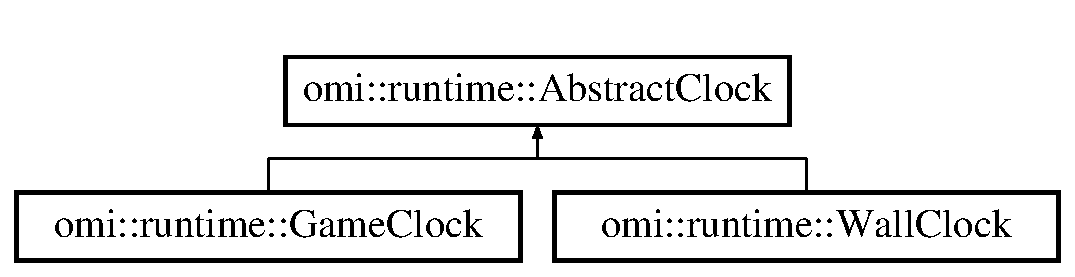
\includegraphics[height=2.000000cm]{classomi_1_1runtime_1_1_abstract_clock}
\end{center}
\end{figure}
\subsection*{Public Types}
\begin{DoxyCompactItemize}
\item 
\hypertarget{classomi_1_1runtime_1_1_abstract_clock_a6af6e30a02165469ffcdcbd512d47a1b}{}enum \hyperlink{classomi_1_1runtime_1_1_abstract_clock_a6af6e30a02165469ffcdcbd512d47a1b}{Metric} \{ {\bfseries M\+E\+T\+R\+I\+C\+\_\+\+N\+A\+N\+O\+S\+E\+C\+O\+N\+D\+S}, 
{\bfseries M\+E\+T\+R\+I\+C\+\_\+\+M\+I\+C\+R\+O\+S\+E\+C\+O\+N\+D\+S}, 
{\bfseries M\+E\+T\+R\+I\+C\+\_\+\+M\+I\+L\+L\+I\+S\+E\+C\+O\+N\+D\+S}, 
{\bfseries M\+E\+T\+R\+I\+C\+\_\+\+S\+E\+C\+O\+N\+D\+S}
 \}\label{classomi_1_1runtime_1_1_abstract_clock_a6af6e30a02165469ffcdcbd512d47a1b}
\begin{DoxyCompactList}\small\item\em Represents the different metrics that clock time can be measured in. \end{DoxyCompactList}
\item 
\hypertarget{classomi_1_1runtime_1_1_abstract_clock_af2122541388aea885afc08e8135340f7}{}typedef arc\+::uint64 \hyperlink{classomi_1_1runtime_1_1_abstract_clock_af2122541388aea885afc08e8135340f7}{time\+\_\+int}\label{classomi_1_1runtime_1_1_abstract_clock_af2122541388aea885afc08e8135340f7}

\begin{DoxyCompactList}\small\item\em Unsigned Integral type used for measuring time. \end{DoxyCompactList}\end{DoxyCompactItemize}
\subsection*{Public Member Functions}
\begin{DoxyCompactItemize}
\item 
\hypertarget{classomi_1_1runtime_1_1_abstract_clock_a36bf3e030ee8096c0be9c85949dd281d}{}\hyperlink{classomi_1_1runtime_1_1_abstract_clock_a36bf3e030ee8096c0be9c85949dd281d}{Abstract\+Clock} ()\label{classomi_1_1runtime_1_1_abstract_clock_a36bf3e030ee8096c0be9c85949dd281d}

\begin{DoxyCompactList}\small\item\em Super constructor. \end{DoxyCompactList}\item 
\hypertarget{classomi_1_1runtime_1_1_abstract_clock_a7c0ab1571043a7475ed2214ec9aaf33a}{}\hyperlink{classomi_1_1runtime_1_1_abstract_clock_a7c0ab1571043a7475ed2214ec9aaf33a}{Abstract\+Clock} (const \hyperlink{classomi_1_1runtime_1_1_abstract_clock}{Abstract\+Clock} \&other)\label{classomi_1_1runtime_1_1_abstract_clock_a7c0ab1571043a7475ed2214ec9aaf33a}

\begin{DoxyCompactList}\small\item\em Super copy constructor. \end{DoxyCompactList}\item 
\hypertarget{classomi_1_1runtime_1_1_abstract_clock_ae09f0723a287c54fa3afeef09d7f4fba}{}\hyperlink{classomi_1_1runtime_1_1_abstract_clock_ae09f0723a287c54fa3afeef09d7f4fba}{Abstract\+Clock} (\hyperlink{classomi_1_1runtime_1_1_abstract_clock}{Abstract\+Clock} \&\&other)\label{classomi_1_1runtime_1_1_abstract_clock_ae09f0723a287c54fa3afeef09d7f4fba}

\begin{DoxyCompactList}\small\item\em Super move constructor. \end{DoxyCompactList}\item 
\hypertarget{classomi_1_1runtime_1_1_abstract_clock_a04cb4c8a300d2d15eef7bc5be43b45ea}{}\hyperlink{classomi_1_1runtime_1_1_abstract_clock}{Abstract\+Clock} \& \hyperlink{classomi_1_1runtime_1_1_abstract_clock_a04cb4c8a300d2d15eef7bc5be43b45ea}{operator=} (const \hyperlink{classomi_1_1runtime_1_1_abstract_clock}{Abstract\+Clock} \&other)\label{classomi_1_1runtime_1_1_abstract_clock_a04cb4c8a300d2d15eef7bc5be43b45ea}

\begin{DoxyCompactList}\small\item\em Assignment operator. \end{DoxyCompactList}\item 
\hypertarget{classomi_1_1runtime_1_1_abstract_clock_ae7b8a8d919d194d1fa063cbce5772d1e}{}\hyperlink{classomi_1_1runtime_1_1_abstract_clock}{Abstract\+Clock} \& \hyperlink{classomi_1_1runtime_1_1_abstract_clock_ae7b8a8d919d194d1fa063cbce5772d1e}{operator=} (\hyperlink{classomi_1_1runtime_1_1_abstract_clock}{Abstract\+Clock} \&\&other)\label{classomi_1_1runtime_1_1_abstract_clock_ae7b8a8d919d194d1fa063cbce5772d1e}

\begin{DoxyCompactList}\small\item\em Move operator. \end{DoxyCompactList}\item 
\hypertarget{classomi_1_1runtime_1_1_abstract_clock_aeacac367a243c33b773b8b06933b1f7b}{}virtual \hyperlink{classomi_1_1runtime_1_1_abstract_clock_a6af6e30a02165469ffcdcbd512d47a1b}{Metric} \hyperlink{classomi_1_1runtime_1_1_abstract_clock_aeacac367a243c33b773b8b06933b1f7b}{get\+\_\+native\+\_\+metric} () const  =0\label{classomi_1_1runtime_1_1_abstract_clock_aeacac367a243c33b773b8b06933b1f7b}

\begin{DoxyCompactList}\small\item\em Returns the highest resolution that this clock natively ticks time at. \end{DoxyCompactList}\item 
\hypertarget{classomi_1_1runtime_1_1_abstract_clock_ab504674ae140328a3a4dd3a2b02b89c8}{}\hyperlink{classomi_1_1runtime_1_1_abstract_clock_af2122541388aea885afc08e8135340f7}{time\+\_\+int} \hyperlink{classomi_1_1runtime_1_1_abstract_clock_ab504674ae140328a3a4dd3a2b02b89c8}{get\+\_\+time} (\hyperlink{classomi_1_1runtime_1_1_abstract_clock_a6af6e30a02165469ffcdcbd512d47a1b}{Metric} metric=M\+E\+T\+R\+I\+C\+\_\+\+M\+I\+L\+L\+I\+S\+E\+C\+O\+N\+D\+S)\label{classomi_1_1runtime_1_1_abstract_clock_ab504674ae140328a3a4dd3a2b02b89c8}

\begin{DoxyCompactList}\small\item\em Returns the current time as an unsigned integral type using the given metric. \end{DoxyCompactList}\item 
double \hyperlink{classomi_1_1runtime_1_1_abstract_clock_a2e4f50f159a450e7f57692c9425f6821}{get\+\_\+multiplier} () const 
\begin{DoxyCompactList}\small\item\em Returns the multiplier being used on the rate of time by this clock. \end{DoxyCompactList}\item 
\hypertarget{classomi_1_1runtime_1_1_abstract_clock_a7d6ea5465b61ada67327f0fbb5fb01d2}{}void \hyperlink{classomi_1_1runtime_1_1_abstract_clock_a7d6ea5465b61ada67327f0fbb5fb01d2}{set\+\_\+multiplier} (double multiplier)\label{classomi_1_1runtime_1_1_abstract_clock_a7d6ea5465b61ada67327f0fbb5fb01d2}

\begin{DoxyCompactList}\small\item\em Sets the multiplier this clock will use on the rate of time. \end{DoxyCompactList}\item 
void \hyperlink{classomi_1_1runtime_1_1_abstract_clock_a2e86653313c678dbd25db870405a89ba}{resume} ()
\begin{DoxyCompactList}\small\item\em Resumes normal ticking of the clock if it has been paused. \end{DoxyCompactList}\item 
\hypertarget{classomi_1_1runtime_1_1_abstract_clock_af5f62abc082be6ee53d4d7a6cf0912a3}{}void \hyperlink{classomi_1_1runtime_1_1_abstract_clock_af5f62abc082be6ee53d4d7a6cf0912a3}{pause} ()\label{classomi_1_1runtime_1_1_abstract_clock_af5f62abc082be6ee53d4d7a6cf0912a3}

\begin{DoxyCompactList}\small\item\em Pauses ticking of the clock. This means the time returned by \hyperlink{classomi_1_1runtime_1_1_abstract_clock_ab504674ae140328a3a4dd3a2b02b89c8}{get\+\_\+time()} will remain unchanged until \hyperlink{classomi_1_1runtime_1_1_abstract_clock_a2e86653313c678dbd25db870405a89ba}{resume()} is called or the clock is manually stepped. \end{DoxyCompactList}\item 
\hypertarget{classomi_1_1runtime_1_1_abstract_clock_ac7674af8453a01e81a929fbd45e871bf}{}bool \hyperlink{classomi_1_1runtime_1_1_abstract_clock_ac7674af8453a01e81a929fbd45e871bf}{is\+\_\+paused} () const \label{classomi_1_1runtime_1_1_abstract_clock_ac7674af8453a01e81a929fbd45e871bf}

\begin{DoxyCompactList}\small\item\em Returns whether this clock is currently paused or not. \end{DoxyCompactList}\item 
void \hyperlink{classomi_1_1runtime_1_1_abstract_clock_acba0e258c160ec6a19477f8558af19d7}{step} (\hyperlink{classomi_1_1runtime_1_1_abstract_clock_af2122541388aea885afc08e8135340f7}{time\+\_\+int} amount, \hyperlink{classomi_1_1runtime_1_1_abstract_clock_a6af6e30a02165469ffcdcbd512d47a1b}{Metric} metric=M\+E\+T\+R\+I\+C\+\_\+\+M\+I\+L\+L\+I\+S\+E\+C\+O\+N\+D\+S)
\begin{DoxyCompactList}\small\item\em Steps the clock by the given amount if the clock is currently paused. \end{DoxyCompactList}\end{DoxyCompactItemize}
\subsection*{Protected Member Functions}
\begin{DoxyCompactItemize}
\item 
virtual \hyperlink{classomi_1_1runtime_1_1_abstract_clock_af2122541388aea885afc08e8135340f7}{time\+\_\+int} \hyperlink{classomi_1_1runtime_1_1_abstract_clock_ace80346afa39d7f7de9c272b1c5f2d25}{tick} ()=0
\begin{DoxyCompactList}\small\item\em Should be implemented by derived classes and returns the current time for the device this clock is using. \end{DoxyCompactList}\end{DoxyCompactItemize}


\subsection{Detailed Description}
Abstract time keeping device. 

This objects provides functionality for modifying the speed of the clock or steeping through clock ticks. For atomic clocks (such as a wall clock or a C\+P\+U cycles clock) this functionality should still be provided for debugging purposes. 

\subsection{Member Function Documentation}
\hypertarget{classomi_1_1runtime_1_1_abstract_clock_a2e4f50f159a450e7f57692c9425f6821}{}\index{omi\+::runtime\+::\+Abstract\+Clock@{omi\+::runtime\+::\+Abstract\+Clock}!get\+\_\+multiplier@{get\+\_\+multiplier}}
\index{get\+\_\+multiplier@{get\+\_\+multiplier}!omi\+::runtime\+::\+Abstract\+Clock@{omi\+::runtime\+::\+Abstract\+Clock}}
\subsubsection[{get\+\_\+multiplier() const }]{\setlength{\rightskip}{0pt plus 5cm}double omi\+::runtime\+::\+Abstract\+Clock\+::get\+\_\+multiplier (
\begin{DoxyParamCaption}
{}
\end{DoxyParamCaption}
) const}\label{classomi_1_1runtime_1_1_abstract_clock_a2e4f50f159a450e7f57692c9425f6821}


Returns the multiplier being used on the rate of time by this clock. 

\begin{DoxyNote}{Note}
Defaults to 1.\+0 
\end{DoxyNote}
\hypertarget{classomi_1_1runtime_1_1_abstract_clock_a2e86653313c678dbd25db870405a89ba}{}\index{omi\+::runtime\+::\+Abstract\+Clock@{omi\+::runtime\+::\+Abstract\+Clock}!resume@{resume}}
\index{resume@{resume}!omi\+::runtime\+::\+Abstract\+Clock@{omi\+::runtime\+::\+Abstract\+Clock}}
\subsubsection[{resume()}]{\setlength{\rightskip}{0pt plus 5cm}void omi\+::runtime\+::\+Abstract\+Clock\+::resume (
\begin{DoxyParamCaption}
{}
\end{DoxyParamCaption}
)}\label{classomi_1_1runtime_1_1_abstract_clock_a2e86653313c678dbd25db870405a89ba}


Resumes normal ticking of the clock if it has been paused. 

If the clock is not currently paused this function does nothing. \hypertarget{classomi_1_1runtime_1_1_abstract_clock_acba0e258c160ec6a19477f8558af19d7}{}\index{omi\+::runtime\+::\+Abstract\+Clock@{omi\+::runtime\+::\+Abstract\+Clock}!step@{step}}
\index{step@{step}!omi\+::runtime\+::\+Abstract\+Clock@{omi\+::runtime\+::\+Abstract\+Clock}}
\subsubsection[{step(time\+\_\+int amount, Metric metric=\+M\+E\+T\+R\+I\+C\+\_\+\+M\+I\+L\+L\+I\+S\+E\+C\+O\+N\+D\+S)}]{\setlength{\rightskip}{0pt plus 5cm}void omi\+::runtime\+::\+Abstract\+Clock\+::step (
\begin{DoxyParamCaption}
\item[{{\bf time\+\_\+int}}]{amount, }
\item[{{\bf Metric}}]{metric = {\ttfamily METRIC\+\_\+MILLISECONDS}}
\end{DoxyParamCaption}
)}\label{classomi_1_1runtime_1_1_abstract_clock_acba0e258c160ec6a19477f8558af19d7}


Steps the clock by the given amount if the clock is currently paused. 

If the clock in not paused this function will have no affect.


\begin{DoxyParams}{Parameters}
{\em amount} & The amount to step the clock by. \\
\hline
{\em metric} & The time metric that the amount parameter represents. \\
\hline
\end{DoxyParams}
\hypertarget{classomi_1_1runtime_1_1_abstract_clock_ace80346afa39d7f7de9c272b1c5f2d25}{}\index{omi\+::runtime\+::\+Abstract\+Clock@{omi\+::runtime\+::\+Abstract\+Clock}!tick@{tick}}
\index{tick@{tick}!omi\+::runtime\+::\+Abstract\+Clock@{omi\+::runtime\+::\+Abstract\+Clock}}
\subsubsection[{tick()=0}]{\setlength{\rightskip}{0pt plus 5cm}virtual {\bf time\+\_\+int} omi\+::runtime\+::\+Abstract\+Clock\+::tick (
\begin{DoxyParamCaption}
{}
\end{DoxyParamCaption}
)\hspace{0.3cm}{\ttfamily [protected]}, {\ttfamily [pure virtual]}}\label{classomi_1_1runtime_1_1_abstract_clock_ace80346afa39d7f7de9c272b1c5f2d25}


Should be implemented by derived classes and returns the current time for the device this clock is using. 

This function should not handle time multipliers or explicit stepping as that will be handled by the \hyperlink{classomi_1_1runtime_1_1_abstract_clock}{Abstract\+Clock} class. 

Implemented in \hyperlink{classomi_1_1runtime_1_1_game_clock_a8c0942d48db3f207b0de2a7ff77bd52e}{omi\+::runtime\+::\+Game\+Clock}, and \hyperlink{classomi_1_1runtime_1_1_wall_clock_a3a7252baf0bd82141aeb60e2303fb56a}{omi\+::runtime\+::\+Wall\+Clock}.



The documentation for this class was generated from the following file\+:\begin{DoxyCompactItemize}
\item 
D\+:/\+Dropbox/\+Development/\+Omicron/\+Omicron/src/cpp/omicron/runtime/clock/Abstract\+Clock.\+hpp\end{DoxyCompactItemize}

\hypertarget{classomi_1_1runtime_1_1_game_clock}{}\section{omi\+:\+:runtime\+:\+:Game\+Clock Class Reference}
\label{classomi_1_1runtime_1_1_game_clock}\index{omi\+::runtime\+::\+Game\+Clock@{omi\+::runtime\+::\+Game\+Clock}}


Clock that measures time since the game engine last started.  




{\ttfamily \#include $<$Game\+Clock.\+hpp$>$}

Inheritance diagram for omi\+:\+:runtime\+:\+:Game\+Clock\+:\begin{figure}[H]
\begin{center}
\leavevmode
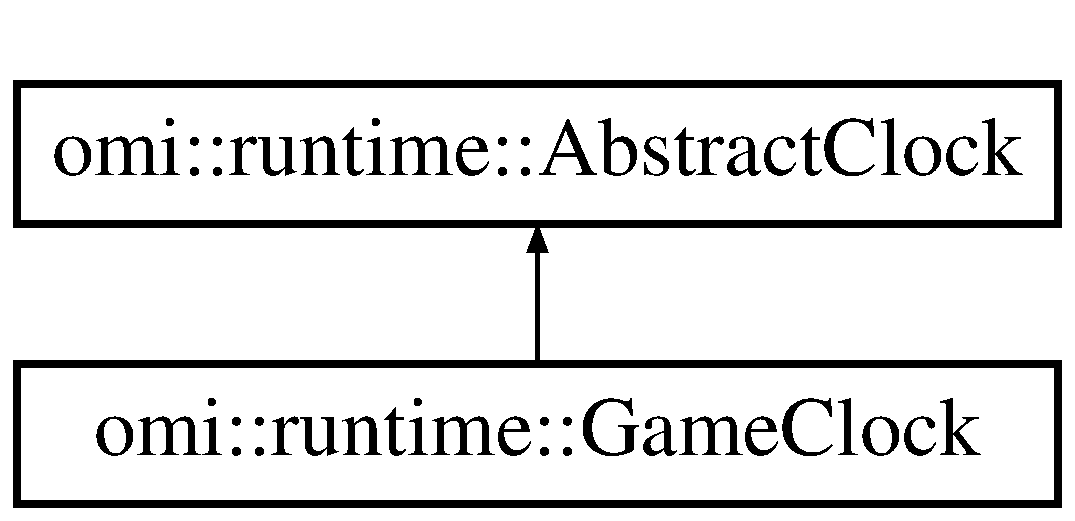
\includegraphics[height=2.000000cm]{classomi_1_1runtime_1_1_game_clock}
\end{center}
\end{figure}
\subsection*{Public Member Functions}
\begin{DoxyCompactItemize}
\item 
virtual \hyperlink{classomi_1_1runtime_1_1_abstract_clock_a6af6e30a02165469ffcdcbd512d47a1b}{Metric} \hyperlink{classomi_1_1runtime_1_1_game_clock_a656c46b8609b36aa109be61413a978c8}{get\+\_\+native\+\_\+metric} () const \hypertarget{classomi_1_1runtime_1_1_game_clock_a656c46b8609b36aa109be61413a978c8}{}\label{classomi_1_1runtime_1_1_game_clock_a656c46b8609b36aa109be61413a978c8}

\begin{DoxyCompactList}\small\item\em Returns the highest resolution that this clock natively ticks time at. \end{DoxyCompactList}\end{DoxyCompactItemize}
\subsection*{Protected Member Functions}
\begin{DoxyCompactItemize}
\item 
\hyperlink{classomi_1_1runtime_1_1_abstract_clock_af2122541388aea885afc08e8135340f7}{time\+\_\+int} \hyperlink{classomi_1_1runtime_1_1_game_clock_a8c0942d48db3f207b0de2a7ff77bd52e}{tick} ()
\begin{DoxyCompactList}\small\item\em Should be implemented by derived classes and returns the current time for the device this clock is using. \end{DoxyCompactList}\end{DoxyCompactItemize}
\subsection*{Additional Inherited Members}


\subsection{Detailed Description}
Clock that measures time since the game engine last started. 

\subsection{Member Function Documentation}
\index{omi\+::runtime\+::\+Game\+Clock@{omi\+::runtime\+::\+Game\+Clock}!tick@{tick}}
\index{tick@{tick}!omi\+::runtime\+::\+Game\+Clock@{omi\+::runtime\+::\+Game\+Clock}}
\subsubsection[{\texorpdfstring{tick()}{tick()}}]{\setlength{\rightskip}{0pt plus 5cm}{\bf time\+\_\+int} omi\+::runtime\+::\+Game\+Clock\+::tick (
\begin{DoxyParamCaption}
{}
\end{DoxyParamCaption}
)\hspace{0.3cm}{\ttfamily [protected]}, {\ttfamily [virtual]}}\hypertarget{classomi_1_1runtime_1_1_game_clock_a8c0942d48db3f207b0de2a7ff77bd52e}{}\label{classomi_1_1runtime_1_1_game_clock_a8c0942d48db3f207b0de2a7ff77bd52e}


Should be implemented by derived classes and returns the current time for the device this clock is using. 

This function should not handle time multipliers or explicit stepping as that will be handled by the \hyperlink{classomi_1_1runtime_1_1_abstract_clock}{Abstract\+Clock} class. 

Implements \hyperlink{classomi_1_1runtime_1_1_abstract_clock_ace80346afa39d7f7de9c272b1c5f2d25}{omi\+::runtime\+::\+Abstract\+Clock}.



The documentation for this class was generated from the following file\+:\begin{DoxyCompactItemize}
\item 
/home/david/\+Dropbox/\+Development/\+Omicron/\+Omicron/src/cpp/omicron/runtime/clock/Game\+Clock.\+hpp\end{DoxyCompactItemize}

\hypertarget{classomi_1_1runtime_1_1_wall_clock}{}\section{omi\+:\+:runtime\+:\+:Wall\+Clock Class Reference}
\label{classomi_1_1runtime_1_1_wall_clock}\index{omi\+::runtime\+::\+Wall\+Clock@{omi\+::runtime\+::\+Wall\+Clock}}


Clock that measures real time from January 1st 1970.  




{\ttfamily \#include $<$Wall\+Clock.\+hpp$>$}

Inheritance diagram for omi\+:\+:runtime\+:\+:Wall\+Clock\+:\begin{figure}[H]
\begin{center}
\leavevmode
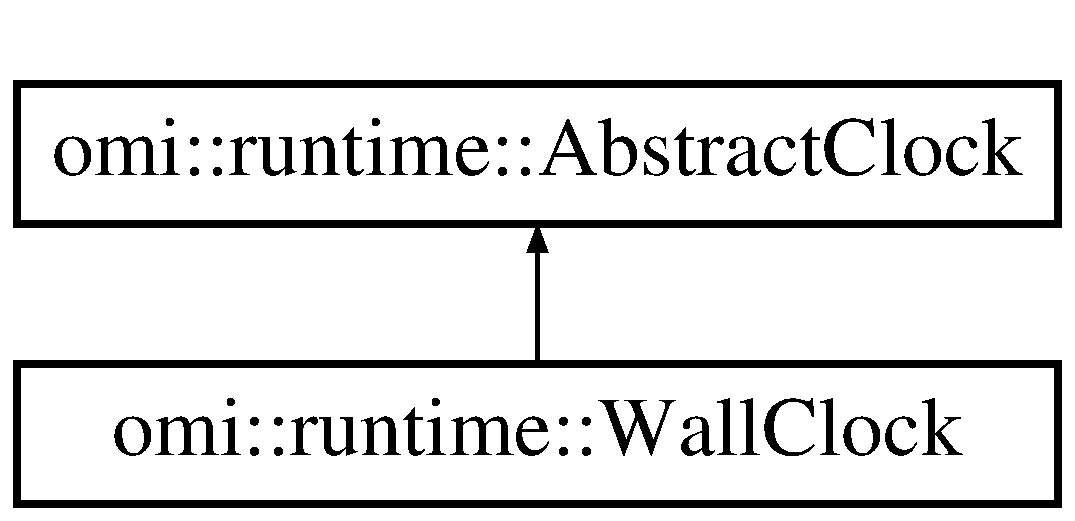
\includegraphics[height=2.000000cm]{classomi_1_1runtime_1_1_wall_clock}
\end{center}
\end{figure}
\subsection*{Public Member Functions}
\begin{DoxyCompactItemize}
\item 
\hypertarget{classomi_1_1runtime_1_1_wall_clock_a275514a3171792b2067eda5cfac9490d}{}virtual \hyperlink{classomi_1_1runtime_1_1_abstract_clock_a6af6e30a02165469ffcdcbd512d47a1b}{Metric} \hyperlink{classomi_1_1runtime_1_1_wall_clock_a275514a3171792b2067eda5cfac9490d}{get\+\_\+native\+\_\+metric} () const \label{classomi_1_1runtime_1_1_wall_clock_a275514a3171792b2067eda5cfac9490d}

\begin{DoxyCompactList}\small\item\em Returns the highest resolution that this clock natively ticks time at. \end{DoxyCompactList}\end{DoxyCompactItemize}
\subsection*{Protected Member Functions}
\begin{DoxyCompactItemize}
\item 
\hyperlink{classomi_1_1runtime_1_1_abstract_clock_af2122541388aea885afc08e8135340f7}{time\+\_\+int} \hyperlink{classomi_1_1runtime_1_1_wall_clock_a3a7252baf0bd82141aeb60e2303fb56a}{tick} ()
\begin{DoxyCompactList}\small\item\em Should be implemented by derived classes and returns the current time for the device this clock is using. \end{DoxyCompactList}\end{DoxyCompactItemize}
\subsection*{Additional Inherited Members}


\subsection{Detailed Description}
Clock that measures real time from January 1st 1970. 

\subsection{Member Function Documentation}
\hypertarget{classomi_1_1runtime_1_1_wall_clock_a3a7252baf0bd82141aeb60e2303fb56a}{}\index{omi\+::runtime\+::\+Wall\+Clock@{omi\+::runtime\+::\+Wall\+Clock}!tick@{tick}}
\index{tick@{tick}!omi\+::runtime\+::\+Wall\+Clock@{omi\+::runtime\+::\+Wall\+Clock}}
\subsubsection[{tick()}]{\setlength{\rightskip}{0pt plus 5cm}{\bf time\+\_\+int} omi\+::runtime\+::\+Wall\+Clock\+::tick (
\begin{DoxyParamCaption}
{}
\end{DoxyParamCaption}
)\hspace{0.3cm}{\ttfamily [protected]}, {\ttfamily [virtual]}}\label{classomi_1_1runtime_1_1_wall_clock_a3a7252baf0bd82141aeb60e2303fb56a}


Should be implemented by derived classes and returns the current time for the device this clock is using. 

This function should not handle time multipliers or explicit stepping as that will be handled by the \hyperlink{classomi_1_1runtime_1_1_abstract_clock}{Abstract\+Clock} class. 

Implements \hyperlink{classomi_1_1runtime_1_1_abstract_clock_ace80346afa39d7f7de9c272b1c5f2d25}{omi\+::runtime\+::\+Abstract\+Clock}.



The documentation for this class was generated from the following file\+:\begin{DoxyCompactItemize}
\item 
D\+:/\+Dropbox/\+Development/\+Omicron/\+Omicron/src/cpp/omicron/runtime/clock/Wall\+Clock.\+hpp\end{DoxyCompactItemize}

%--- End generated contents ---

% Index
\backmatter
\newpage
\phantomsection
\clearemptydoublepage
\addcontentsline{toc}{chapter}{Index}
\printindex

\end{document}
